\documentclass{article}

% If you're new to LaTeX, here's some short tutorials:
% https://www.overleaf.com/learn/latex/Learn_LaTeX_in_30_minutes
% https://en.wikibooks.org/wiki/LaTeX/Basics

% Formatting
\usepackage[utf8]{inputenc}
\usepackage[margin=1in]{geometry}
\usepackage[titletoc,title]{appendix}

% Math
% https://www.overleaf.com/learn/latex/Mathematical_expressions
% https://en.wikibooks.org/wiki/LaTeX/Mathematics
\usepackage{amsmath,amsfonts,amssymb,mathtools}

% Images
% https://www.overleaf.com/learn/latex/Inserting_Images
% https://en.wikibooks.org/wiki/LaTeX/Floats,_Figures_and_Captions
\usepackage{graphicx,float}

% Tables
% https://www.overleaf.com/learn/latex/Tables
% https://en.wikibooks.org/wiki/LaTeX/Tables

% Algorithms
% https://www.overleaf.com/learn/latex/algorithms
% https://en.wikibooks.org/wiki/LaTeX/Algorithms
\usepackage[ruled,vlined]{algorithm2e}
\usepackage{algorithmic}

% Code syntax highlighting
% https://www.overleaf.com/learn/latex/Code_Highlighting_with_minted
\usepackage{minted}
\usemintedstyle{borland}

% References
% https://www.overleaf.com/learn/latex/Bibliography_management_in_LaTeX
% https://en.wikibooks.org/wiki/LaTeX/Bibliography_Management
\usepackage{biblatex}
\addbibresource{references.bib}

\usepackage{enumitem}

% Title content
\title{CS6910 : Deep Learning (for Computer Vision)}
\author{\textbf{Irfaan Arif} \\ {\textbf{ME18B048}}}
\date{\textbf{Assignment 3}}

\begin{document}

\maketitle
\vspace{-1.6em}

% Introduction and Overview
\section{Part-A : }
\subsection*{Train and Test your own Word2Vec}

For this part we have to train our own Word2Vec model for the 'text8'  dataset. The following models as described in class were implemented
\begin{enumerate}[label=(\alph*),noitemsep]
    \item Bag-of-words
    \item Skip-gram
    \item LSTM-based models
\end{enumerate}
The python script (nlppreprocessing.py) given in Moodle was used to preprocess the dataset.\\

\noindent
 All experiments and results below are on the outputs of the proprocessing script on the 'text8' dataset. The models were trained on a AWS instance (g4dn.xlarge)  with varying training parameters. The model with the best validation accuracy among all the epochs was taken as the result for each experiment. \\

\noindent
For each of these, in the word\_to\_idx generated from the text8 vocabulary, the index '0' is reserved for words which we might come across later but arent there in the vocabulary, 'OOV' words. Our train vocabulary size made from the 'text8' dataset is 253702.

\subsubsection*{Bag of words}
For this we are using the continuous bag of words approach. The CBOW model architecture tries to predict the current target word (the center word) based on the source context words (the surrounding words with a window size). The model used is attached as Figure \ref{fig:cbow_model}. We are using nn.NLLLoss on logsoftmaxed outputs with SGD as the optimizer, after training the loss plateaued to around \textbf{2.80}

\begin{figure}[H]
    \centering
    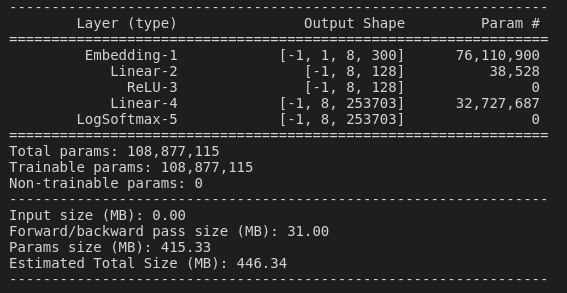
\includegraphics[width=0.60\linewidth]{models/cbow_model.png}
    \caption{The CBOW model with window size 4}
    \label{fig:cbow_model}
\end{figure}

\subsubsection*{Skip-gram}

Skip-gram on the other hand is used to predict the context word for a given target word. It’s the reverse of CBOW algorithm. Here, target word is input and the context words are output. The model used is attached as Figure \ref{fig:skipgram_model}. For this skipgram implementation we are using 2 different embedding layers for the context and target, and both are trainable. For skipgram we take negative of the logsigmoid of the embedding product as the loss and SGD as the optimizer again, after training the total loss came to about \textbf{3.15}. We will be experimenting using both in Part B.

\vspace{3.0em}

\begin{figure}[H]
    \centering
    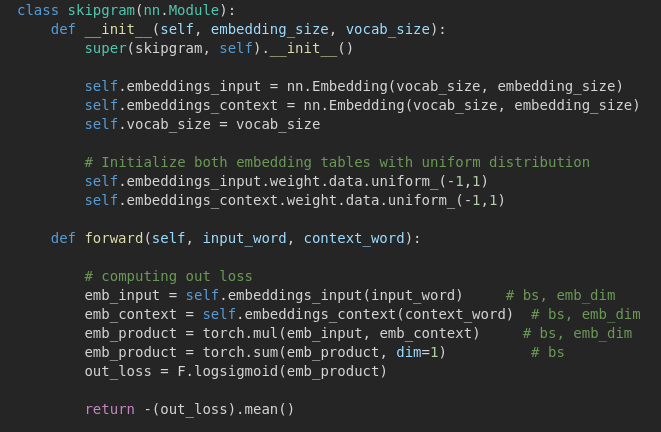
\includegraphics[width=0.60\linewidth]{models/skipgram_model.png}
    \caption{The Skipgram model}
    \label{fig:skipgram_model}
\end{figure}


\begin{figure}[H]
    \centering
    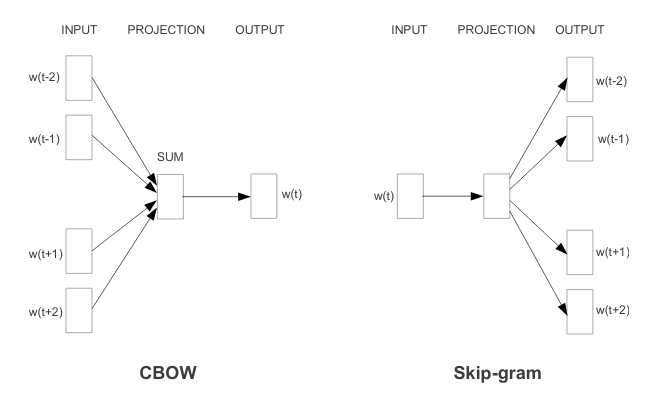
\includegraphics[width=0.80\linewidth]{cbow_vs_skipgram.png}
    \caption{CBOW vs skipgram (source: arXiv:1301.3781)}
    \label{fig:comaprison_model}
\end{figure}
\subsubsection*{LSTM-based models}

For LSTM-based model, we can define the training task to predict a target word given context words before it, similar to what is done in the CBOW model. Here we take a target word as the output and try to predict it given window\_size words before it as input. The model used is attached as Figure \ref{fig:lsmt_q1_model}. We are again using nn.NLLLoss on the logsoftmaxed outputs with Adam as the optimizer, after training the loss plateaued to around \textbf{1.40}
\begin{figure}[H]
    \centering
    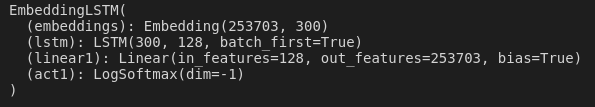
\includegraphics[width=0.60\linewidth]{models/lstm_model.png}
    \caption{LSTM-based model}
    \label{fig:lsmt_q1_model}
\end{figure}


\section{Part-B : }
\subsection*{Sentiment Analysis in movie reviews}

The task given was to classify movie reviews in one of the 5 classes based on the sentiment of the review.  We are to make a feature representation of the review using pre-trained word embedding \& our own embedding which were trained in  Part-A and use an LSTM based model to classify to one of the 5 classes mentioned below.  

The sentiment labels are:
\begin{itemize}[noitemsep]
    \item 0 - negative 
    \item 1 - somewhat negative
    \item 2 - neutral 
    \item 3 - somewhat positive
    \item 4 - positive
\end{itemize}
 
\subsubsection*{Using pre-trained word embeddings}

The following 4 pre-trained word embeddings were used from the torchtext library
\begin{itemize}[noitemsep]
    \item FastText - 'simple' - 300 dim
    \item GloVe - '6B' - 100 dim
    \item GloVe - '840B' - 300 dim
    \item FastText - 'en' - 300 dim
\end{itemize}    

\noindent
For all of these pre-trained word embeddings, experiments were run with different models such as by varying the number of LSTM layers, hidden dim, etc. The best results have only been included in this report. Also in the Embeddings layer for all the models, index '0' was reserved for words which might not not be in our vocabulary 'OOV' words. This is because some words in val.csv and test.csv might be missing from our vocabulary made from train.csv
\\


\noindent 
And there were words in our vocabulary for which pre-trained word embeddings were not available (ref Table \ref{tab:miss_words}). For these few words, a random vector was initialized from the normal distribution (scale of 0.6). The same is also done for index '0' of our embedding weight matrix. For every other word for which an embedding was available, it was copied to the embedding weight matrix. Our vocabulary made from the reviews in train.csv had 15136 words.\\
\newpage

\begin{table}[h!]
\begin{center}
\begin{tabular}{ |c|c|c|c|} 
 \hline
 Pre-trained word embedding & Word embeddings found & Words embeddings missing  & \%found\\ 
 \hline \hline
 FastText - 'simple' & 12072 & 3064  & 79.83\\ 
 \hline
 GloVe - '6B' & 14742  & 394 & 97.39  \\ 
\hline
 GloVe - '840B' & 14742  & 394  & 97.39\\ 
\hline
 FastText - 'en' & \textbf{14845}  & 291  & \textbf{98.08}\\

\hline
\end{tabular}
\caption{Pre-trained word Embeddings availability }
\label{tab:miss_words}
\end{center}
\end{table}


\noindent 
Experiments were run in which the embeddings weights were frozen and also in which they were also trainable. The results are tabulated below in Table \ref{tab:results_pretrained} \& \ref{tab:classwise_results_pretrained}. The model used for the experiments is attached as Figure \ref{fig:best_model} \\

\begin{table}[h!]
\begin{center}
\begin{tabular}{ |c|c||} 
 \hline
 Pre-trained word embedding & \%Test Accuracy\\ 
 \hline \hline
 FastText - 'simple' & 59.93\\ 
 \hline
 FastText - 'simple' - frozen & 60.34 \\ 
 \hline
 GloVe - '6B' &  61.30 \\ 
\hline
 GloVe - '6B' - frozen &  62.00 \\ 
\hline
 GloVe - '840B' & 63.01 \\
\hline
 GloVe - '840B' - frozen & \textbf{63.77} \\
\hline
 FastText - 'en' & 62.53 \\
 \hline
 FastText - 'en' - frozen & 62.81 \\
\hline
\end{tabular}
\caption{Test accuracy for each model }
\label{tab:results_pretrained}
\end{center}
\end{table}

\begin{table}[h!]
\begin{center}
\begin{tabular}{ |c|c|c|c|c|c|} 
 \hline
 Pre-trained word embedding & 0 & 1 & 2 & 3 & 4\\ 
 \hline \hline
 FastText - 'simple' & \textbf{20.17} & 42.61 & 77.1 & 52.5 & 19.99 \\ 
 \hline
  FastText - 'simple' - frozen & 0.0 & 54.58 & 74.42 & 60.94 & 0.0 \\
 \hline
 GloVe - '6B' & 0.0 & 58.01 & 74.89 & \textbf{61.49} & 0.0 \\
\hline
 GloVe - '6B' - frozen & 16.97 & 52.68 & 77.19 & 59.97 & 0.14 \\
 \hline
 GloVe - '840B' & 14.7 & 54.49 & 78.11 & 61.33 & 0.94 \\
\hline
 GloVe - '840B' - frozen & 7.73 & 57.91 & \textbf{78.85} & 51.02 & \textbf{39.54} \\
 \hline
 FastText - 'en' & 1.32 & \textbf{60.84} & 76.71 & 60.23 & 0.14 \\
  \hline
 FastText - 'en' - frozen & 0.0 & 55.78 & 78.23 & 52.91 & 34.03 \\  


\hline
\end{tabular}
\caption{Class wise accuracy for each }
\label{tab:classwise_results_pretrained}
\end{center}
\end{table}

\begin{figure}[H]
    \centering
    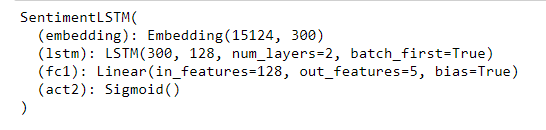
\includegraphics[width=0.7\linewidth]{model_lstm_q2.png}
    \caption{LSTM model used}
    \label{fig:best_model}
\end{figure}

\noindent
Figures 6 to 21 have the model accuracy's over training and confusion matrix's for each of the pre-trained word embeddings with both the embedding layers frozen and trainable.
\newpage

\begin{itemize}

    \item FastText 'simple'
    \begin{figure}[H]
    \centering
    \begin{minipage}{.5\linewidth}
        \centering
        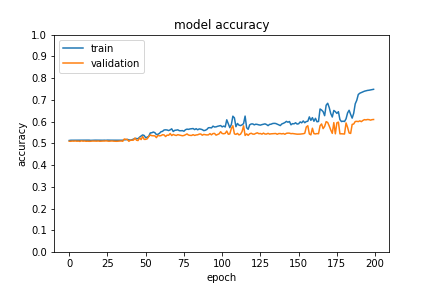
\includegraphics[width=0.9\linewidth]{pre_trained_res/train_fast_simple_frozen.png}
        \vspace{-1.0em}
        \caption{Embedding layer frozen}

    \end{minipage}%
    \begin{minipage}{.5\textwidth}
      \centering
      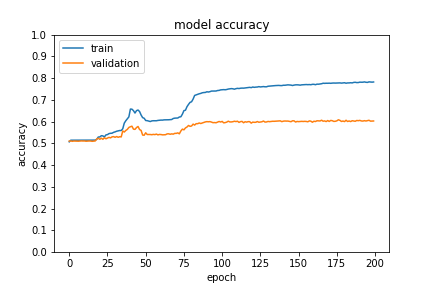
\includegraphics[width=.9\linewidth]{pre_trained_res/train_fast_simple.png}
      \vspace{-1.0em}
      \caption{Embedding layer trainable}

    \end{minipage}
    \end{figure}
    \begin{figure}[H]
    \centering
    \begin{minipage}{.5\linewidth}
        \centering
        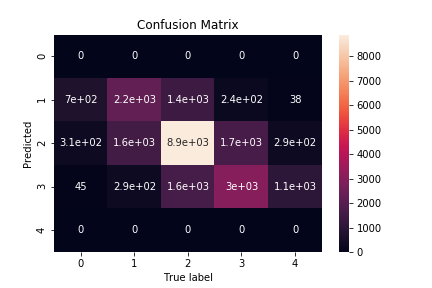
\includegraphics[width=1.2\linewidth]{pre_trained_res/cm_fast_simple_frozen.png}
        \vspace{-2.2em}
        \caption{Embedding layer frozen}

    \end{minipage}%
    \begin{minipage}{.5\textwidth}
      \centering
      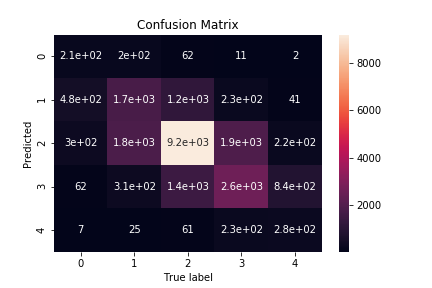
\includegraphics[width=1.2\linewidth]{pre_trained_res/cm_fast_simple.png}
      \vspace{-2.2em}
      \caption{Embedding layer trainable}

    \end{minipage}
    \end{figure}
    
    \item GloVe - '6B'
    \begin{figure}[H]
    \centering
    \begin{minipage}{.5\linewidth}
        \centering
        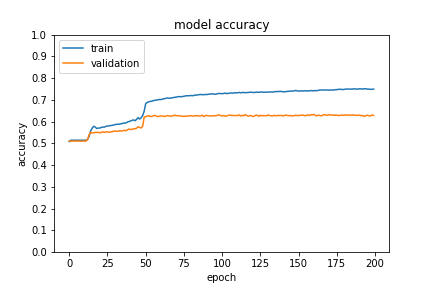
\includegraphics[width=0.9\linewidth]{pre_trained_res/train_glove_6_frozen.png}
        \vspace{-1.0em}
        \caption{Embedding layer frozen}

    \end{minipage}%
    \begin{minipage}{.5\textwidth}
      \centering
      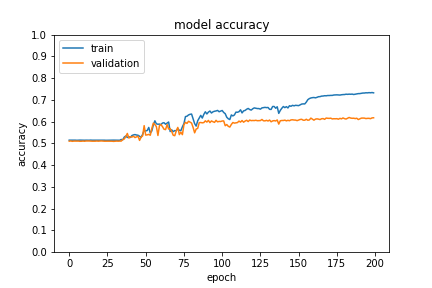
\includegraphics[width=.9\linewidth]{pre_trained_res/train_glove_6.png}
      \vspace{-1.0em}
      \caption{Embedding layer trainable}

    \end{minipage}
    \end{figure}
        \begin{figure}[H]
    \centering
    \begin{minipage}{.5\linewidth}
        \centering
        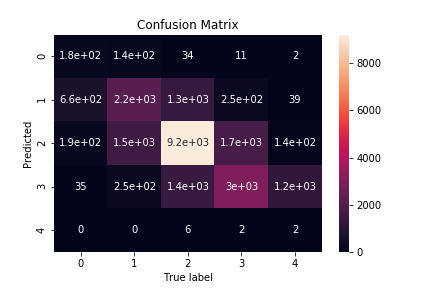
\includegraphics[width=1.2\linewidth]{pre_trained_res/cm_glove_6_ frozen.png}
        \vspace{-2.2em}
        \caption{Embedding layer frozen}

    \end{minipage}%
    \begin{minipage}{.5\textwidth}
      \centering
      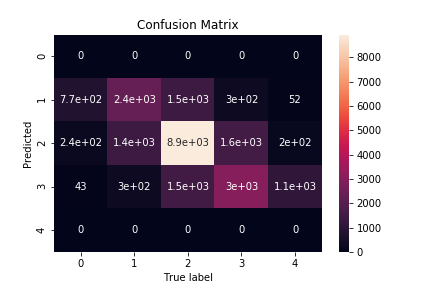
\includegraphics[width=1.2\linewidth]{pre_trained_res/cm_glove_6.png}
      \vspace{-2.2em}
      \caption{Embedding layer trainable}

    \end{minipage}
    \end{figure}
    
    \item GloVe - '840B'
    \begin{figure}[H]
    \centering
    \begin{minipage}{.5\linewidth}
        \centering
        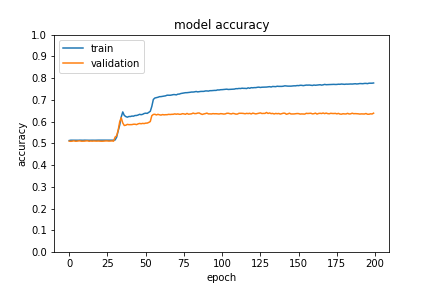
\includegraphics[width=0.9\linewidth]{pre_trained_res/train_glove_840_frozen.png}
        \vspace{-1.0em}
        \caption{Embedding layer frozen}

    \end{minipage}%
    \begin{minipage}{.5\textwidth}
      \centering
      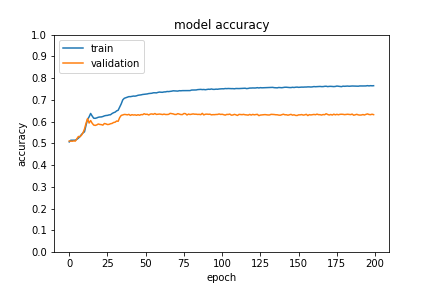
\includegraphics[width=.9\linewidth]{pre_trained_res/train_glove_840.png}
      \vspace{-1.0em}
      \caption{Embedding layer trainable}

    \end{minipage}
    \end{figure}
        \begin{figure}[H]
    \centering
    \begin{minipage}{.5\linewidth}
        \centering
        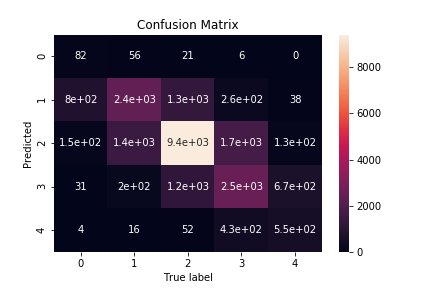
\includegraphics[width=1.2\linewidth]{pre_trained_res/cm_glove_840_ frozen.png}
        \vspace{-2.2em}
        \caption{Embedding layer frozen}

    \end{minipage}%
    \begin{minipage}{.5\textwidth}
      \centering
      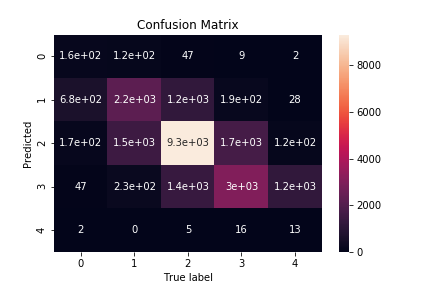
\includegraphics[width=1.2\linewidth]{pre_trained_res/cm_glove_840.png}
      \vspace{-2.2em}
      \caption{Embedding layer trainable}

    \end{minipage}
    \end{figure}
    
    \newpage
    \item FastText - 'en'
    \begin{figure}[H]
    \centering
    \begin{minipage}{.5\linewidth}
        \centering
        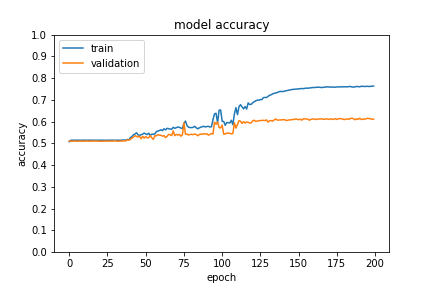
\includegraphics[width=0.9\linewidth]{pre_trained_res/train_fast_en_frozen.png}
        \vspace{-1.0em}
        \caption{Embedding layer frozen}

    \end{minipage}%
    \begin{minipage}{.5\textwidth}
      \centering
      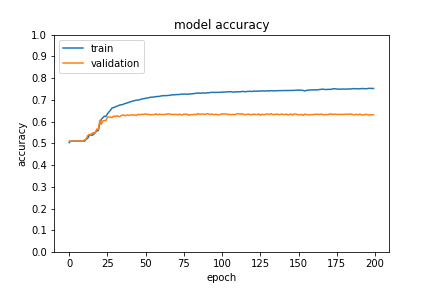
\includegraphics[width=.9\linewidth]{pre_trained_res/train_fast_en.png}
      \vspace{-1.0em}
      \caption{Embedding layer trainable}

    \end{minipage}
    \end{figure}
    \begin{figure}[H]
    \centering
    \begin{minipage}{.5\linewidth}
        \centering
        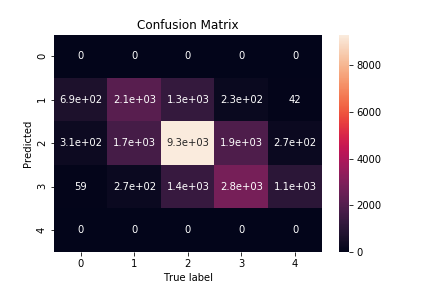
\includegraphics[width=1.2\linewidth]{pre_trained_res/cm_fast_en_frozen.png}
        \vspace{-2.2em}
        \caption{Embedding layer frozen}

    \end{minipage}%
    \begin{minipage}{.5\textwidth}
      \centering
      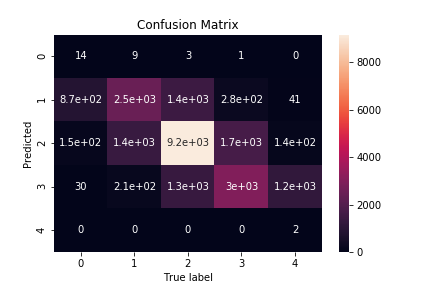
\includegraphics[width=1.2\linewidth]{pre_trained_res/cm_fast_en.png}
      \vspace{-2.2em}
      \caption{Embedding layer trainable}

    \end{minipage}
    \end{figure}
\end{itemize}

\noindent
As can be seen from the accuracy tables and the confusion matrices, the model have very good performance for neutral category and relatively good performance for the somewhat negative and somewhat positive categories. Most of the models tend to find it hard to categorize the completely positive and negative reviews. Also since not many embedings were found in the FastText - ’simple’ pre trained embedding, it as expected had the worst performance among these pre-trained word embeddings. Between the GloVe pre-trained word embeddings, since '6B' only had 100 dim embedding space compared to '840B' having 300 dim, GloVe '840' had better performance.\\

\noindent
It is to note that the there were more number of reviews for the neutral category and the slighly positive and negative classes in the train.csv file as seen in table \ref{tab:dataset_imbalance}, this also leads to our models to lean towards predicting these majority classes as the training accuracy would be higher, as this is a training class-imbalance problem, techniques like under-sampling, minority oversampling could be used to take care of this.
\begin{table}[h!]
\begin{center}
\begin{tabular}{ |c|c|c|c|c|c|} 
 \hline
 Train data classes  & 0 & 1 & 2 & 3 & 4\\ 
 \hline \hline
Number of train samples & 4650 & 18443 & 54488 & 22327 & 6086\\ 
\hline
Percentage of dataset & 0.044 &\textbf{0.174} & \textbf{0.514} &\textbf{0.211} &0.057 \\

\hline
\end{tabular}
\caption{Train dataset class imbalance }
\label{tab:dataset_imbalance}
\end{center}
\end{table}
\\

\noindent
As a result the size of the embedding dimension and the number of word embeddings available for our vocabulary are the major factors to consider when selecting a pre-trained word embedding to use.



\subsubsection*{Using embeddings from the models in Part A}

For each of the models trained in Part A, the word\_to\_idx dictionary was pickled and stored, also the weights of the embeddings layer in the models were also extracted and stored in a .npz compressed format. Now for every word in the vocabulary from train.csv, if the word in present in the loaded word\_to\_idx dictionary, then the trained embedding was used and copied to the weight matrix. The words for which embeddings were not available, a random vector was initialized from the normal distribution (scale of 0.6).The same is also done for index ’0’ of our embedding weight matrix for out of vocabulary 'OOV' words that might appear during validation and testing.\\

\begin{table}[h!]
\begin{center}
\begin{tabular}{ |c|c|c|c|} 
 \hline
 Word embedding from & Word embeddings found & Words embeddings missing  & \%found\\ 
 \hline \hline
 Vocab from 'text8' & 13832 & 1291  & \textbf{91.46}\\ 
 \hline

\hline
\end{tabular}
\caption{Word Embeddings availability }
\label{tab:miss_words1}
\end{center}
\end{table}
\vspace{-1.6em}
\noindent
The model is used for the experiments below is basically the same as the one used when we were using pre-trained embeddings. It is attached as Figure \ref{fig:model_used_q2}.

\begin{figure}[H]
    \centering
    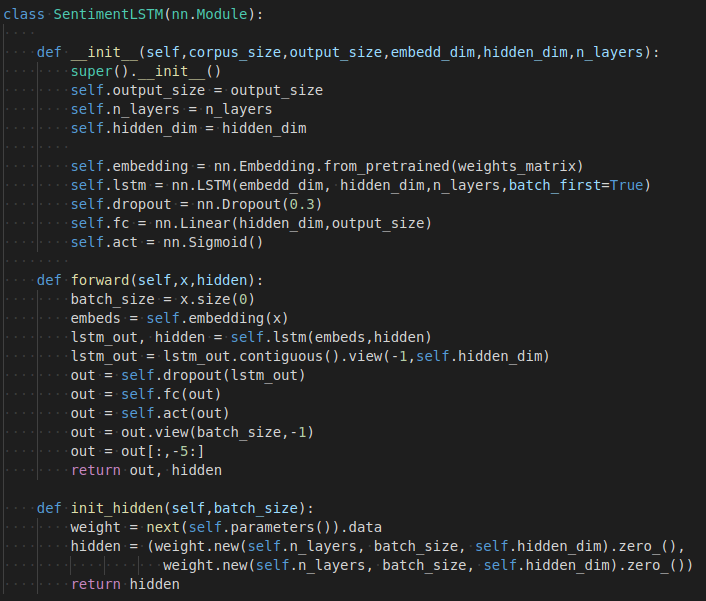
\includegraphics[width=0.80\linewidth]{model_q2.png}
    \caption{LSTM model used}
    \label{fig:model_used_q2}
\end{figure}

\noindent
Figures attached below have the model accuracy's over training and confusion matrix's for each of the models by which word embeddings have been trained in Part A. For these models we have kept the weights frozen from what we got from Part A.
\newpage


\begin{itemize}[noitemsep]
    \item CBOW model
    \vspace{-1.0em}
    \begin{figure}[H]
    \centering
    \begin{minipage}{.5\linewidth}
        \centering
        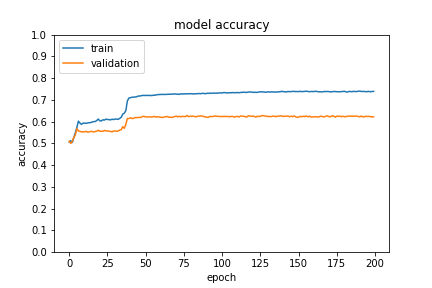
\includegraphics[width=1.1\linewidth]{trained_From_q1/train_cbow.png}
        \vspace{-1.0em}

    \end{minipage}%
    \begin{minipage}{.5\textwidth}
      \centering
      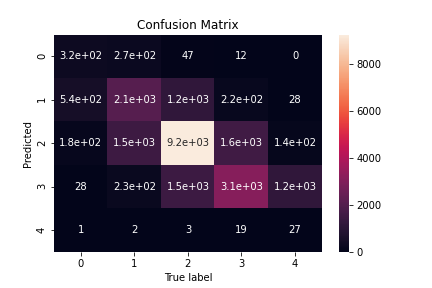
\includegraphics[width=1.2\linewidth]{trained_From_q1/cm_cbow.png}
      \vspace{-1.0em}

    \end{minipage}
    \end{figure}
    
    \vspace{-1.0em}
    \item Skipgram
    \vspace{-1.0em}
    \begin{figure}[H]
    \centering
    \begin{minipage}{.5\linewidth}
        \centering
        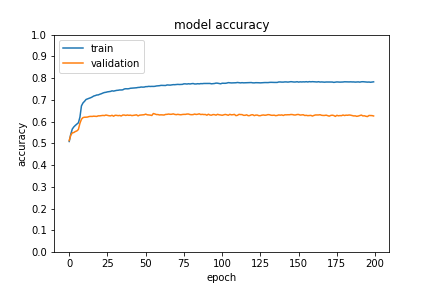
\includegraphics[width=1.1\linewidth]{trained_From_q1/train_skipgram.png}
        \vspace{-1.0em}

    \end{minipage}%
    \begin{minipage}{.5\textwidth}
      \centering
      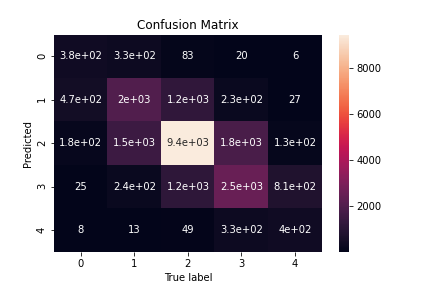
\includegraphics[width=1.2\linewidth]{trained_From_q1/cm_skipgram.png}
      \vspace{-1.0em}

    \end{minipage}
    \end{figure}
    
    \vspace{-1.0em}
    \item LSTM based model
    \vspace{-1.0em}   
    \begin{figure}[H]
    \centering
    \begin{minipage}{.5\linewidth}
        \centering
        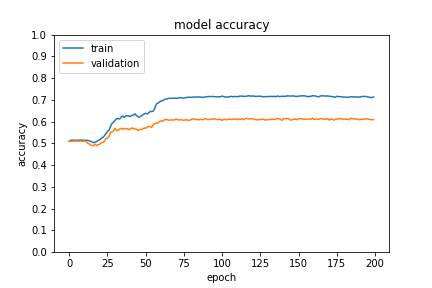
\includegraphics[width=1.1\linewidth]{trained_From_q1/train_lstm.png}
        \vspace{-1.0em}

    \end{minipage}%
    \begin{minipage}{.5\textwidth}
      \centering
      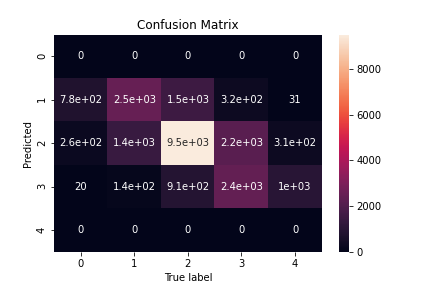
\includegraphics[width=1.2\linewidth]{trained_From_q1/cm_lstm.png}
      \vspace{-1.0em}

    \end{minipage}
    \end{figure}
    
\end{itemize}

\newpage
\noindent
The relevant metrics for these experiments for each of the models have also been attached in Table \ref{tab:results_q1} and Table \ref{tab:classwise_results_1}

\begin{table}[h!]
\begin{center}
\begin{tabular}{ |c|c||} 
 \hline
Model based on & \%Test Accuracy\\ 
 \hline \hline
CBoW & \textbf{63.78}\\ 
 \hline
Skipgram & 63.17  \\ 
\hline
LSTM - based & 61.60 \\
\hline
\end{tabular}
\caption{Test accuracy for each model }
\label{tab:results_q1}
\end{center}
\end{table}

\vspace{-2.0em}

\begin{table}[h!]
\begin{center}
\begin{tabular}{ |c|c|c|c|c|c|} 
 \hline
Model based on  & 0 & 1 & 2 & 3 & 4\\ 
 \hline \hline
CBoW & 29.78  & 50.57  & 77.44  &\textbf{ 63.43}  & 1.96  \\
 \hline
Skipgram &  \textbf{36.0}  & 48.86  & 79.01  & 51.27  & \textbf{29.18} \\ 
\hline
LSTM - based & 0.0  & \textbf{61.38 } & \textbf{79.53}  & 48.94  & 0.0  \\
\hline
\hline
\end{tabular}
\caption{Class wise accuracy for each }
\label{tab:classwise_results_1}
\end{center}
\end{table}
\vspace{-3.0em}

\subsection*{Conclusions}
After all the experiments the main parameters that seems to affect the accuracy's of our models are:
\begin{enumerate}
    \item \textbf{Embedding dimension} of the embedding layer
    
    For pre-trained embedding the embedding dimension available seems to be directly correlated to the amount of data used to create it, as a result higher the embedding dimension, better the accuracy as discussed before in its section. 
    
    For the model in Part A, it seems that bigger the embedding dimension the better the results obtained from using it in Part B for sentiment classification. The results have been tabulated in Table \ref{tab:emb_dim_res}. As the embedding dimension increases the training time drastically increases especially for a large dataset like 'text8' with very minimal improvements in accuracy, hence only 3 values were tested with.
    \begin{table}[h!]
    \begin{center}
    \begin{tabular}{ |c|c|} 
     \hline
    Embedding dimension  & \% Accuracy \\ 
     \hline \hline
    100 &   61.20\\
     \hline
    300 &   63.02\\ 
    \hline
    500  & 63.78\\
    \hline
    \hline
    \end{tabular}
    \caption{Accuracy for varying embedding dimension (CBoW model was used) }
    \label{tab:emb_dim_res}
    \end{center}
    \end{table}
    
    \item \textbf{Sequence length} of input to the LSTM 
    
    As the input to the LSTM must be fixed, we either truncate long review vector or pad short review vectors with 0 to achieve the sequence length we specify. The results have been tabulated in Table \ref{tab:seq_len_res}. Here also as the sequence length increases the accuracy does increase however after a while you reach the point of very little gain from further increases. Note that all very short and long reviews were also completely excluded from the training process since it would just be bad training data.
    
    \begin{table}[h!]
    \begin{center}
    \begin{tabular}{ |c|c|} 
     \hline
    Seq length  & \% Accuracy \\ 
     \hline \hline
    4 &   54.67\\
     \hline
    8 &   63.78\\ 
    \hline
    12  & 63.83\\
    \hline
    \hline
    \end{tabular}
    \caption{Accuracy for varying sequence lengths (CBoW model was used) }
    \label{tab:seq_len_res}
    \end{center}
    \end{table}
    
    \newpage
    \item \textbf{Window sizes} for each model in Part-A 
        \begin{itemize}
            \item \textbf{CBoW model} 
            
            For the cbow model, here window size refers to the number of context words around the middle target word used to predict it. The results of varying the window size are attached in Table \ref{tab:cbow_ws}
                \begin{table}[h!]
                \begin{center}
                \begin{tabular}{ |c|c|} 
                 \hline
                Window size  & \% Accuracy \\ 
                 \hline \hline
                2 &   60.67\\
                 \hline
                4 &   63.78\\ 
                \hline
                6  &\textbf{ 63.83}\\
                \hline
                \hline
                \end{tabular}
                \caption{Accuracy for varying window size in CBoW }
                \label{tab:cbow_ws}
                \end{center}
                \end{table}
            \item \textbf{Skipgram model}

            
            In the skipram implementation, window size refers to how many context words around the target word are taken to use as training data. The table below, \ref{tab:skipgram_ws} shows the results of varying this window size.

                \begin{table}[h!]
                \begin{center}
                \begin{tabular}{ |c|c|} 
                 \hline
                Window size  & \% Accuracy \\ 
                 \hline \hline
                4 &   \textbf{63.17}\\
                 \hline
                8 &   63.06\\ 
                \hline
                10  & 62.91\\
                \hline
                \hline
                \end{tabular}
                \caption{Accuracy for varying window size in Skipgram }
                \label{tab:skipgram_ws}
                \end{center}
                \end{table}            
            \item \textbf{LSTM based model} 
            
            In the case of LSTM based models, as we have treated it like a word prediction problem, here window size refers to how many words before the target we take to predict the last word. Table \ref{tab:_wslstm} show the results obtained by varying this window size.

                \begin{table}[h!]
                \begin{center}
                \begin{tabular}{ |c|c|} 
                 \hline
                Window size  & \% Accuracy \\ 
                 \hline \hline
                2 &   59.33\\
                 \hline
                4 &   \textbf{61.60}\\ 
                \hline
                6  & 61.56\\
                \hline
                \hline
                \end{tabular}
                \caption{Accuracy for varying window size in LSTM based model }
                \label{tab:_wslstm}
                \end{center}
                \end{table}   
            
        \end{itemize}
\end{enumerate}


\end{document}



